\documentclass[a4paper, 11pt]{article}
\usepackage{comment}
\usepackage{lipsum} 
\usepackage{fullpage} 
\usepackage{graphicx}
\usepackage[margin=1in]{geometry} 
\usepackage{makeidx}
\usepackage{float}
\usepackage{amsmath,amsthm,amssymb, multicol, array}

 
\newcommand{\N}{\mathbb{N}}
\newcommand{\Z}{\mathbb{Z}}

\makeindex



\begin{document}  
\title{SOEN-6611\\ Software Measurement\\ Project Deliverable - I\\ Team - A}

\date{}
\maketitle
\noindent
\begin{minipage}[H]{0.7\textwidth}
\begin{flushleft} \large
\emph{Team Members:}\\
 Nazanin AhmadyShahpourAbady(40086734)
 \\
 Priyanka Anantha Padmanabhan(40040066)
 \\
 Maryam Ansari Sadrabadi(40021574)
 \\
 Rahul Reddy Ayyapaneni(40071075)
 \\
 Mitra Azari Sissi(40021574)
 \\
 Divyeshkumar Balar(40062267)
 \\
 Nikitha Papani(40070806)
 
\end{flushleft}
\end{minipage}
~
\begin{minipage}{0.3\textwidth}
\begin{flushright} \large
\emph{Guided by:} \\
Dr. Pankaj Kamthan
\\
Samia Hilal % Supervisor's Name
\end{flushright}
\end{minipage}\\[2cm]

\begin{center}
	\date{\LARGE June 15, 2018}
\end{center}

\begin{figure}[H]
	
\includegraphics[scale=1]{concordia_logo.png}
	\vspace{1cm}
\end{figure}

\newpage
\tableofcontents
\listoffigures
\listoftables

\newpage
\section{Introduction}
The Process of Software Measurement has been integrated with Software Engineering and depends on the global environment characteristics such as improvement, control, structuring, estimation, and analysis. Software Measurement is like a computation in any other behavior, it will obey the value of measurement if it obtains a wide range of \textbf{Acceptance and Validity}. This is the extremely beneficial effect on the principles of measurement in the subject. The empirical study of software measurement will emphasize the advantages and disadvantages of metrics that have been used and also validate the work of metric. The context related to the software development will act as an important role in the risk management because the metrics which are integrated into a predictive model will give predictive warning messages to the potential risks. To predict a software measurement process, different models, approaches, and standards are required. \\

\section{Assumptions}
\begin{itemize}
\item It is assumed that customer survey includes all necessary questions required for GQM for proposed metric set.
\item It is also assumed that required past artifacts of products are available(Project documentation, Organization source code).
\end{itemize}



\section{Objective}
The main objective of this Software Measurement project is to provide \textbf{DESCRIPTIVE STATISTICS}\cite{1} generation of random numbers. The DESCRIPTIVE STATISTICS will acknowledge the coefficients in a descriptive manner and illustrates the available data set. The required calculations such as mean, median and mode will obtain the measurement of center of distribution and retrieve the maximum number, minimum number and standard deviation will include the \textbf{measure of variability}. The source code of this project has been developed in R language.

\section{GOAL-QUESTION-METRIC}
The Software Measurement considered should be meaningful because almost in every software project time is the major resource to make the effective measurement. It requires a meaningful methodology which is called GQM (Goal Question Metric) approach\cite{2} which is completely based on the goal. This Goal based approach will be the deciding factor for choosing data on which the measurement has to performed and the reason behind the measurement. GQM reveals the structure in the hierarchy, in which goals are finalized in the initial stages and the relationship between the goal to questions and questions to metrics are one-to-many. After deciding on the goal, relevant questions and related metrics will be generated. The goal should provide a statement for an achievement with some measurements.\\
\newpage
\section{GOAL}
Customer Service Manager wants to \textbf{Improve the Customer Satisfaction} of the product by \textbf{analyzing} obtained data from the DESCRIPTIVE STATISTICS on recent customer feedback. \\


\begin{table}[H]
\centering
\label{GQMDef}
\begin{tabular}{|l|}
\hline
\textbf{\begin{tabular}[c]{@{}l@{}}Purpose: To analyze the customer survey/feedback, in order to improve the overall \\ customer satisfaction.\\ \\ Perspective: Examine the usability from the view-point of the user and examine \\reliability and maintainability from the view-point of service manager.\\ \\ Environment: In the context of the maintainance and quality assurance phase from \\the life cycle.\end{tabular}} \\ \hline
\end{tabular}
\caption{GQM Definition}
\end{table}
\subsection{SUB-GOAL 1: Usability}
Question 1: What is the estimated number of defects in the software?\\ \\
Question 2: The Defect removal efficiency of the product?\\ \\ 
Metric 1:Defect removal efficiency\cite{10}
\begin{equation*}
 DRE = \frac{E}{(E+D)}     
\end{equation*}
 where,  \\
E= Errors before product delivery \\
       	D= Errors from end user after product delivery\\ \\
Question 3: How effective is the software in completing a given task?\\ \\
Metric 2: Effectiveness\cite{10}\cite{11} 
\begin{equation*}
    Effectiveness = \frac{Number of tasks completed successfully}{Total  number of tasks undertaken}X100%
\end{equation*}\\ \\
Question 4: How efficient is our software in terms of task-time?\\ \\
Metric 3: Time Based Efficiency\cite{12}
 	\begin{equation*}
    Time Based Efficiency = \frac{\sum_{i=1}^{R} \sum_{j=1}^{N} \frac{n_ij}{t_ij}}{NR}
\end{equation*}\\ \\ 
N = The total number of tasks (goals)\\
R = The number of users\\
Nij = The result of task i by user j; if the user successfully completes the task, then Nij = 1, if not, then Nij = 0.\\
Tij = The time spent by user j to complete task i. If the task is not successfully completed, then time is measured till the moment the user quits the task.\\ \\
Question 5: What is the satisfaction level of users of the software after a certain task?\\  \\
Metric 4: Customer Satisfaction\cite{11}
\begin{equation*}
    CSat = \frac{Sum of all Score}{Number of Respondents}X10
\end{equation*}\\ \\
Question 6: What is the error rate of certain task performed by users who have accessed the software?\\  \\
Metric 5: Net Promoter Score\cite{11}
\begin{equation*}
    Net Promoter Score = \frac{Promoter-Detractor}{Total Respondents}
\end{equation*}\\ \\
Question 7: What is the extent that customer is able to utilize the existing features in the software?\\ \\
Metric 6: Product Utilization Factor\\ \\
"Analyzed and Designed theoretically by DivyeshKumar Balar and Rahul Reddy Ayyapaneni"
\begin{equation*}
    Product Utilization Factor = \frac{Average Number of Feature utilized by the customers}{Total number of available features in the softwares}
\end{equation*}\\ \\

\subsection{SUB-GOAL 2 : Maintainability}

Question 8: Is your code Simple?\\  \\
Question 9: Is code structured well?\\ \\
Metric 7: Customer Satisfaction
Control Flow Complexity = E - N + 2\\
	Where, \\
		E= total number of arcs\\
		N= total number of nodes
\\ \\
Metric 8: LOD - Lack of documentation\cite{10}
\begin{equation*}
     LOD(c) = 1 - \frac{|D(c)|}{|T(c)|}
 \end{equation*}
 Where,
 
 $D(c) = \{ e \in T(c) |e.has RDoc == true\}$
 
 
 $T(C) = Succ(c, containsMethod) \cup c$
 
 Where, $c \in Scope^{LOD}$\\ \\
Question 10: What is level of abstraction of source code?\\ \\
Metric 9: DIT - Depth of Inheritance\cite{9}
\begin{equation*}
    DIT(c) = Max(dist(c,P(c)))    
 \end{equation*}\\
 Where,\\
 $P(c) = Pred^*(c,Inheritance^{DIT})$ Set of classes,c inherits directly or indirectly\\ \\

\subsection{SUB-GOAL 4: Reliability}
Question 11: What is the Product(Application/Software) crash rate?\\ \\
Metric 10: Application Crash Rate\cite{13}
\begin{equation*}
    Average Crash Rate = \frac{Total Number of Failure}{Total Number of Attempt}
\end{equation*}\\ \\
Question 12: What is System’s \textbf{dependability}? \\ \\
Metric 11: Dependability\cite{14} 
\begin{equation*}
     Dependability = 1 - Probability  of failure
 \end{equation*}\\
 Where, Probability of failure is \textbf{mean crash rate}(ACR).\\ \\
Question 13: Is your system \textbf{fault tolerant}?\\ \\ 
Metric 12: Instability\cite{8}
 \begin{equation*}
     Instability(I) = \frac{Ce}{Ce+Ca}
 \end{equation*}
 Where,\\ 
 
 $Ce = Efferent Coupling$
 $Ca = Afferent Coupling$ \\ \\
Question 14: Is your code \textbf{consistent} (In logical order)? \\ \\
Metric 13: LCOM - Lack of Cohesion\cite{8}
 \begin{equation*}
     LCOM^* = \frac{\frac{1}{a}[\sum_{i=1}^{a}\mu(A_i)]-m}{1-m}
 \end{equation*}\\
 Where,\\
 $a$ is number of attributes and $m$ is number of methods\\ \\



\section{Use case Model}
A Use case diagram is an \textbf{extension of UML} it is similar in behavior to UML, which are standard indications for modeling real-world objects and systems. Use case diagrams will standardize the functionality of the system based on actors, who are people or objects handling under predefined responsibilities in a system and relevant Use cases. The physical overview of use case is a combination of actions, services, and functions that the system has to perform. Basically, Use case diagram illustrates a sequence in a combination of actions that results in an \textbf{outcome of measurable} value for an object and it is obtained as a horizontal ellipse. \\
The Use case diagram consists of the following major components:\\
1. It describes the \textbf{relationship} between the actors and Use cases.\\
2. The Use cases, which are the \textbf{major roles of the actors} within the system.\\
3. The actors try to \textbf{involve individually} within the system and act according to their respective roles.\\
4. The margin defines the interest of the system related to the environment.\\ \\

Our Use case diagram consists of \textbf{two actors} namely customer and customer service manager. The use case present for the customer is getData and the use case for customer service manager is sample data. With the help of these two use cases Descriptive Statistics has been generated which included Max.val, Min.val, Mean.val, Median.val, Mode.val, Standard Deviation.\\ \\ 
\begin{figure}[!hbt]
		% Center the figure.
		\begin{center}
		% Include the eps file, scale it such that it's width equals the column width. You can also put width=8cm for example...
		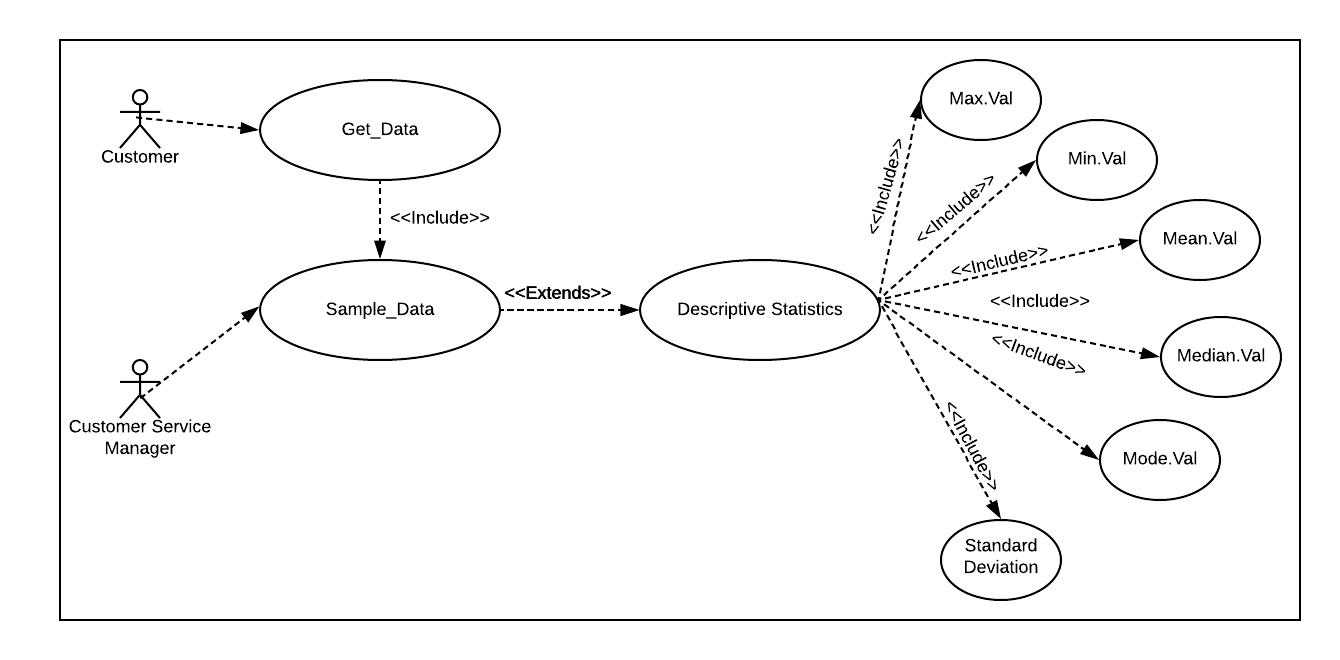
\includegraphics[width=\columnwidth]{Blank_Diagram.png}
		% Create a subtitle for the figure.
		\caption{Use Case Approach}
		% Define the label of the figure. It's good to use 'fig:title', so you know that the label belongs to a figure.
		\label{fig:figure}
		\end{center}
	\end{figure}
%-------------------------------------------------
\begin{table}[H]
\centering
\label{my-label}
\begin{tabular}{|l|l|}
\hline
\textbf{Use Case Model:} & On demand DESCRIPTIVE STATISTICS(DS) \\ \hline
\textbf{Brief Description:} & \begin{tabular}[c]{@{}l@{}}The Input values will be selected randomly from \\ the online customer satisfaction survey\end{tabular} \\  \hline
\textbf{Actor:} & Customer Service Manager, Customer \\ \hline
\textbf{PreConditions:} & Do Customer Survey \\ \hline
\textbf{PostConditions:} & Save the result of DS into database for future use. \\ \hline
\textbf{Trigger:} & Customer Service Manager(CSM) will request to run the DS. \\  \hline
\textbf{Program Scenario:} & \begin{tabular}[c]{@{}l@{}}1.User performs survey and feed data to organizations database \\ 2.Systems request the required quantity input from database and \\    retrive in random order. \\ 3.CSM will trigger the DS to run on that sample data.\\ 4.developed R based system obtain results for Maximum, Minimum,\\    Mean, Median, Mode,Arithmetic Mean and Standard Deviation and \\    other mathematical expressions. 5.System Display statistical data for\\    respected measurements.\end{tabular} \\ \hline
\end{tabular}
\caption{Use Case Description}
\end{table}

%-------------------------------------------------
    
    
    
    
\section{Project Effort Estimation}
\subsection{Use case Points (UCP) Approach:}
The UCP approach will \textbf{estimate the cost and effort} for a Software Measurement project based on the prediction values of the size of the software system.\cite{3} The process of the estimation for effort for a software project is \textbf{much complex} in the initial stages of the software development life cycle where the details of the specific requirements are not clearly defined. There are multiple enhanced optimization techniques which are available to improve the accuracy in effort of a software project. The number of use case points in a software project is totally based on the complexity of the use cases available in the system and also based on the complexity of the actor in the system.\\ \\
The UCP approach will be determined from four the following variables:\\ \\
1.Technical Complexity Factor (TCF)\\
2.Environment Complexity Factor (ECF)\\
3.Unadjusted Use Case Points (UUCP)\\
4.Productivity Factor (PF)\\ \\
From the output values of the above variables, the Effort estimation of a software system will result. The equation of the effort estimation is given by:\\
\begin{equation}
Effort Estimation (E) = UCP * PF = UUCP * TCF * ECF * PF 
\end{equation}
Where, \\
UCP = Use Case Points \\
PF = Productivity Factor \\
UUCP = Unadjusted Use Case Points \\
TCF = Technical Complexity Factor \\
ECF = Environment Complexity Factor \\
\subsubsection{Technical Complexity Factor (TCF)}
To make the effort estimation reliable, we should consider the technical factors, representing relative weights of the factors. There are 13 technical factors for the estimation of use case points approach. Technical complexity factors are designated with a value from 0 to 5 with respect to perceived complexity. The below values of the perceived complexity denotes:\\ \\
0 - Irrelevant\\
3 - Average\\
5 - Strong Influence\\ \\
These 13 technical factors will contribute the complexity of a software project according to the given weights in the below table:\\ \\
Special user training facilities are required.
The Calculated Factor is the combination of weight of the Technical complexity factor and Perceived complexity.\\ 

\begin{table}[ht]
\centering
\footnotesize
\label{TCF}
\begin{tabular}{|c|l|c|c|c|}
\hline
\textbf{Factor} & \textbf{Description} & \textbf{Weight} & \textbf{\begin{tabular}[c]{@{}c@{}}Percieved \\ complexity\end{tabular}} & \textbf{\begin{tabular}[c]{@{}c@{}}Calculated\\ Factor\end{tabular}} \\ \hline
\textbf{T1}     & Distributed System & 2 & 5 & 10                     \\ \hline
\textbf{T2}     & \begin{tabular}[c]{@{}l@{}}Response time or throughput\\ performance objectives\end{tabular} & 1 & 4 & 4 
\\ \hline
\textbf{T3}     & End user efficiency & 1 & 2 & 2                     \\ \hline
\textbf{T4}     & Complex internal processing & 1 & 3 & 3 
\\ \hline
\textbf{T5}     & Code must be reusable & 1 & 4 & 4                   \\ \hline
\textbf{T6}     & Easy to install & 0.5 & 5 & 2.5                     \\ \hline
\textbf{T7}     & Easy to use & 0.5 & 3 & 1.5                         \\ \hline
\textbf{T8}     & Portable & 2 & 2 & 4                               \\ \hline
\textbf{T9}     & Easy to change & 1 & 5 & 5 \\ \hline
\textbf{T10}    & Concurrent & 1 & 1 & 1                             \\ \hline
\textbf{T11}    & Includes special security objectives & 1 & 2 & 2
\\ \hline
\textbf{T12}    & Provides direct access for third parties& 1 & 4 &4 \\ \hline
\textbf{T13}    & Special user training facilities are required & 1 & 3  & 3                                                             \\ \hline
\end{tabular}
\caption{TCF Calculation}
\end{table}




Calculated Factor = Weight * Perceived Complexity\\

Then the Total Factor  =  45\\
\begin{equation}
TCF = C1 + (C2 * Total Factor)
\end{equation}


Since the actor is Complex actor, we should consider assign the maximum values for the constants C1 and C2\\

Then C1 = 0.6 and C2 = 0.01\\ \\
TCF = .60 + (0.01 * Total Factor)\\
        = .60 + (0.01 * 45)\\
        = .60 + 0.45\\
        = 1.05\\
Hence The Technical Complexity Factor \textbf{TCF  = 1.05}\

\subsubsection{Environment Complexity Factor (ECF)}
Environment complexity factor will estimate the \textbf{impact on the productivity} on \textbf{multiple environmental variable} factors which are existing in a software project.\cite{3} There are eight environment complexity factor and representing with weight factors. 

\begin{table}[ht]
\centering
\footnotesize
\label{my-label}
\begin{tabular}{|c|l|c|c|c|}
\hline
\textbf{Environmental Factor} & \textbf{Description}           & \textbf{Weight} & \textbf{\begin{tabular}[c]{@{}c@{}}Percieved \\ complexity\end{tabular}} & \textbf{\begin{tabular}[c]{@{}c@{}}Calculated\\ Factor\end{tabular}} \\ \hline
\textbf{E1} & Familiarity with UML & 1.5 & 4 & 6                     \\ \hline
\textbf{E2} & Application Experience & 0.5 & 2 & 1                   \\ \hline
\textbf{E3} & Object Oriented Experience & 1 & 3 & 7                 \\ \hline
\textbf{E4} & Lead analyst capability & 0.5 & 2 & 1                 \\ \hline
\textbf{E5} & Motivation & 1 & 5                                                                        & 5                                                                    \\ \hline
\textbf{E6}                   & Stable Requirements            & 2               & 4                                                                        & 8                                                                    \\ \hline
\textbf{E7}                   & Part-time workers              & -1              & 1                                                                        & -1                                                                   \\ \hline
\textbf{E8}                   & Difficult Programming language & 2               & 1                                                                        & 1                                                                    \\ \hline
\end{tabular}
\caption{ECF Calculation}
\end{table}

\textbf{The Environment Total Factor = 28}\\
Since for ECF C1 = 1.4 and C2 = -0.03\\
ECF = C1 + (-0.03 * Total Factor)\\
    = 1.4 + (-0.03 * 28)\\
                 = 1.4 - 0.84\\
                 = 0.56\\
\textbf{ECF = 0.56}
\subsubsection{Unadjusted Use case Point (UUCP)}
Unadjusted Use Case is the combination of two basic variables.\\
UUCW = \textbf{U}nadjusted \textbf{U}se \textbf{C}ase \textbf{W}eight which consists total number of steps in use case process.
UAW = \textbf{U}nadjusted \textbf{A}ctor \textbf{W}eight which is derived on the basis the complexity of the use case actors.\\

\subsubsection{Unadjusted Actor Weight (UAW)}
The UAW is measured on the basis of number of actors available in the software system and combining the result with weight of the particular actor.\\ \\

\begin{tabular}{| >{\centering\arraybackslash}m{1in} | >{\centering\arraybackslash}m{1in} | >{\centering\arraybackslash}m{1in} | >{\centering\arraybackslash}m{1in} |>{\centering\arraybackslash}m{1in} |}
\hline 
  \textbf{Actor Type} & \textbf{Use Case Type} & \textbf{Weight} & \textbf{No of Use cases} &\textbf{Results} \\[8pt]
  \hline
  Simple & Simple & 1 & 0 & 0 \\[8pt]
  \hline
  Average & Average &2 & 1 & 2 \\[8pt]
  \hline
  Complex & Complex &3 & 0 & 0 \\[8pt]
  \hline
\end{tabular} \\ \\

\textbf{Total UAW = 2}

\subsubsection{Unadjusted Use case Weight (UUCW)}
The Unadjusted use case weight is estimated based on number of use cases available in the software system per each category and also by combining the value of use case along with actor weight.\\ \\

\begin{tabular}{| >{\centering\arraybackslash}m{1in} | >{\centering\arraybackslash}m{1in} | >{\centering\arraybackslash}m{1in} | >{\centering\arraybackslash}m{1in} |>{\centering\arraybackslash}m{1in} |}
\hline 
  \textbf{Use Case Type} & \textbf{Description Weight} & \textbf{Weight} & \textbf{No of Use cases} &\textbf{Results} \\[8pt]
  \hline
  UC1 & Simple Use Case & 5 & 0 & 0 \\[8pt]
  \hline
  UC2 & Average Use Case &10 & 1 & 10 \\[8pt]
  \hline
  UC3 & Complex Use Case &15 & 0 & 0 \\[8pt]
  \hline
\end{tabular} \\ \\ \\
Then the Total \textbf{UUCW = 10}\\
Hence calculate the Unadjusted Use case points\\
\textbf{UUCP} = UUCW + UAW = 10 + 2 = \textbf{12}.\\	

\subsubsection{Productivity Factor (PF)}
The productivity is defined as the ratio of the number of man hours per use case scenario based on the previous software projects.\\
There will be a default value for the productivity factor is \textbf{20}.\\

Hence the Use case points UCP = TCF * ECF * UUCP 
                                                    =  1.05 * 0.56 * 12
                                                    =  7.056

Then from the value of \textbf{UCP = 7.056}, calculate Effort.

\textbf{Effort Estimation} = UCP * PF
                           = 7.056 * 20 = \textbf{141.12 Person-Hours}

\subsection{COCOMO 81 (COCOMO I)}
The COCOMO 81 which is also called constructive estimation cost model is a fundamental method of \textbf{cost evaluation} of a software projects.\cite{3} The software projects are classified into three classes:\\ \\
1.Organic Projects\\
2.Semi-Detached\\
3.Embedded\\

\subsubsection{Organic Projects}
The Organic mode projects are \textbf{comparatively smaller and simpler software} projects. This is because these simple software projects contain a small team with good application experience. The organic projects look similar to the previously developed projects which require less amount of innovation.\\ 

\subsubsection{Semi-Detached}
The semi-detached projects are \textbf{intermediate in size and complexity} in the context of the software projects in which the teams have mixed experience levels must meet a mix of unaltered and less than immutable requirements.\\

\subsubsection{Embedded}
This is a type of software project which is developed under \textbf{very strong requirements} and a set of transparent hardware and software constraints.

The given equation for the basic COCOMO calculation is:

\begin{equation*}
    Effort =  a(S)^{b} * F\\
\end{equation*}
a,b = coefficients\\
	S   = Size of the system\\
    F   = Adjustment Factor = 1\\ \\

\begin{figure}[!hbt]
		% Center the figure.
		\begin{center}
		% Include the eps file, scale it such that it's width equals the column width. You can also put width=8cm for example...
		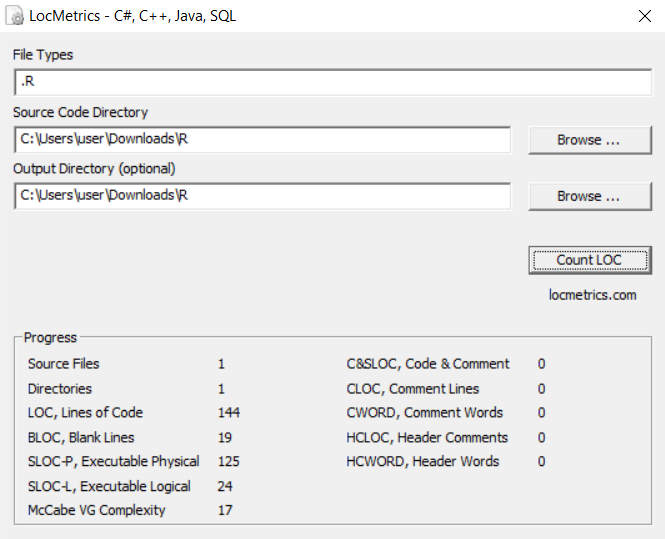
\includegraphics[width=\columnwidth]{LOC.PNG}
		\caption{Lines of Code From LOCMetrics}
		\label{fig:figure}
		\end{center}
	\end{figure}

The below is the tabular information regarding coefficients of COCOMO\\

\begin{tabular}{| >{\centering\arraybackslash}m{1in} | >{\centering\arraybackslash}m{1in} | >{\centering\arraybackslash}m{1in} | >{\centering\arraybackslash}m{1in} |>{\centering\arraybackslash}m{1in} |}
\hline 
  \textbf{Development Mode} & \textbf{a} & \textbf{b} & \textbf{c} &\textbf{d} \\
  \hline
  Organic & 2.4 & 1.05 & 2.5 & 0.38 \\[8pt]
  \hline
  Semi-Detached & 3 &1.12 & 2.5 & 0.35 \\[8pt]
  \hline
  Embedded & 3.6 &1.2 & 2.5 & 0.32 \\[8pt]
  \hline
\end{tabular} \\ 

\begin{equation*}
   \textbf{ Effort} = \frac{ a(S)^{b} * F}\\
           = \frac{3.0 (0.179) ^ {1.12} * 1}\\
           = \textbf{0.436 Person-Month}
\end{equation*}

Let’s consider \textbf{1 Person-Month = 176 Person-Hours}\\

Because the user will be working \textbf{22 days in a month}, \textbf{8 hours per day}.\\

Then Effort\textbf{ E} = .436 * 176 = \textbf{77 Person-Hours}\\ \\
This has been concluded from the above two different evaluations of effort estimation with Use case point approach and COCOMO calculation. The difference between Use case points approach and basic \textbf{COCOMO calculation} is \textbf{45 Percentage}. The use case point approach indicated 141 person-hours which are more predictive and relevant. COCOMO has given the result of 77 person-hours, which is less than use case point approach.\\
It is a better way to go with an \textbf{overestimation} since the development mode is semi-detached, which is a mixed level of experiences as well as with rigid requirements.\\


\section{Cyclomatic Complexity Number}
The concept of the Cyclomatic complexity indicates the level of complexity of the source code. The measurement of Cyclomatic complexity revolves around two variables.\cite{6}\\ \\
Nodes = n\\
Edges = e \\
The given equation for cyclomatic complexity is:\\
\begin{equation}
V(G) = e - n + 2
\end{equation}
Through this calculation, we can identify for the features like, whether the source code of the program is compatible with testing or not, is it able to understand the logic that exists in the source code and whether the source code is reliable. There are multiple cyclomatic complexity levels according to the risk management.\\ \\ \\

  1 - 10  = Low - Simple Control flow graph  \\

  11 - 20  = Moderate - Complex control flow graph  \\

  21 - 50  = High - Complex, but manageable control flow graph  \\

  Greater Than 50  = Very Strong - Very Complex, unmanageable control flow graph.\\
The cyclomatic complexity of the DESCRIPTIVE STATISTICS are provided below along with control flow graphs.\\
\footnotesize
\begin{figure}[H]
		\begin{center}
		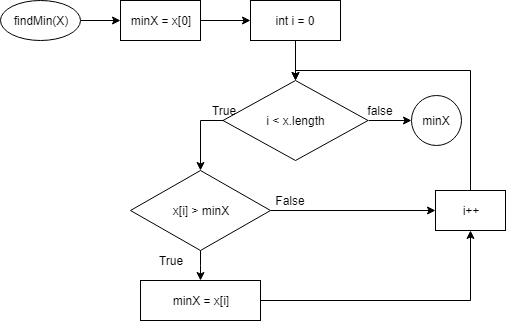
\includegraphics[width=\columnwidth]{MIN.png}
		\caption{Control flow graph for Minimum Number}
		\label{fig:figure}
		\end{center}
	\end{figure}
The Cyclomatic complexity = e - n + 2 = 9 - 8 + 2 = 3\\
\begin{figure}[H]
		\begin{center}
		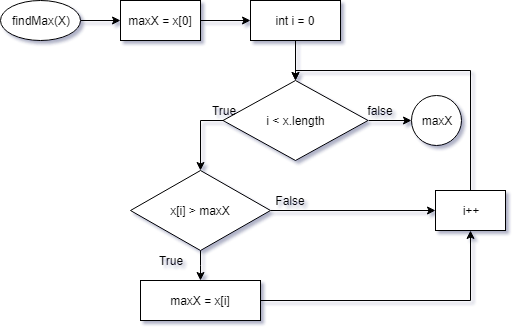
\includegraphics[width=\columnwidth]{Max_controlFlow.png}
		\caption{Control flow graph for Maximum Number}
		\label{fig:figure}
		\end{center}
	\end{figure}
The cyclomatic complexity = e - n + 2 = 9 - 8 + 2 = 3\\ \\
\begin{figure}[H]
		\begin{center}
		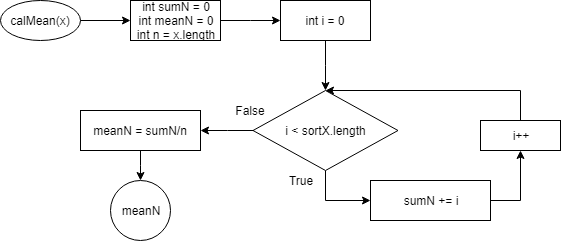
\includegraphics[width=\columnwidth]{mean_controlFlow.png}
		\caption{Control flow graph for Mean}
		\label{fig:figure}
		\end{center}
	\end{figure}
The Cyclomatic complexity = e - n + 2 = 8 - 8 + 2 = 2\\
\begin{figure}[H]
		\begin{center}
		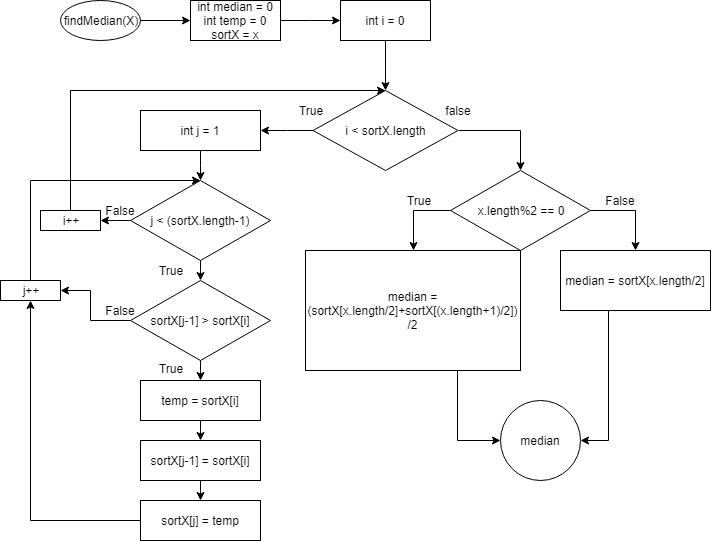
\includegraphics[width=\columnwidth]{median_controlFlow.png}
		\caption{Control flow graph for Median}
		\label{fig:figure}
		\end{center}
	\end{figure}
The Cyclomatic complexity  = e - n + 2 = 19 - 16 + 2 = 5\\
\begin{figure}[H]
		\begin{center}
		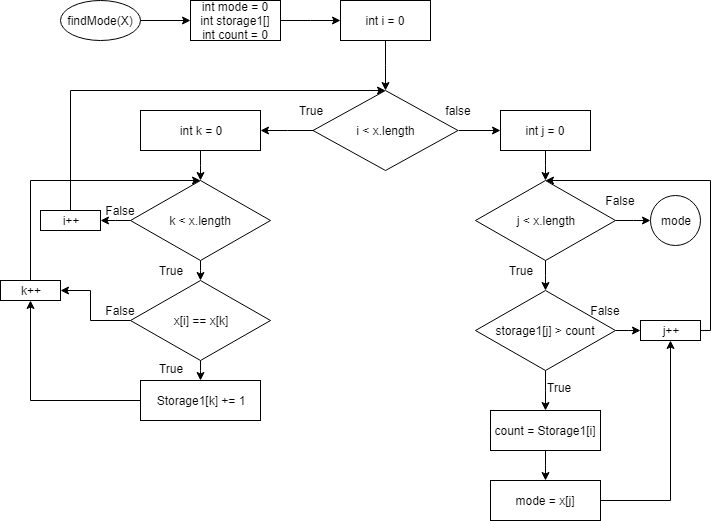
\includegraphics[width=\columnwidth]{mode_controlFlow.png}
		\caption{Control flow graph for Mode}
		\label{fig:figure}
		\end{center}
	\end{figure}
The Cyclomatic complexity = e - n + 2 = 21 - 17 + 2 = 6\\
\begin{figure}[H]
		\begin{center}
		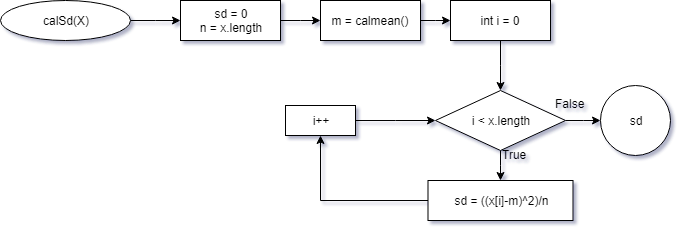
\includegraphics[width=\columnwidth]{sd_controlFlow.png}
		\caption{Control Flow Graph for Standard Deviation}
		\label{fig:figure}
		\end{center}
	\end{figure}

The Cyclomatic Complexity = e - n + 2 = 8 - 8 + 2  = 2\\



\section{Object-Oriented Metrics WMC, CF and LCOM*}
The Object-Oriented Metrics Paradigm for assessing the system has become widely used in order to produce high-quality results. For measuring the quality of Object-Oriented Software, Chidamber and Kemerer software metrics suite was developed in the year 1994. C and K initially developed  six metrics which were widely accepted by the Software Development Community. ‘Weighted Methods per Class (WMC)’ and ‘Lack of Cohesion in methods (LCOM*)’ are the metrics of that suite. ‘Coupling Factor (CF)’ is one of the six metrics of the Metrics for Object Oriented Design (MOOD Suite) given by Fernando Brito and Rogerio Carpuca in 1994.\cite{9}\\

\subsection{Weighted Methods per Class (WMC)}
WMC calculates the sum of \textbf{complexities of all methods} in a class. It is used to estimate the time and effort needed to develop and maintain a class. \\

\begin{equation*}
WMC = \sum_{i=1}^{k} {C_i}
\end{equation*}
where, 
	i= $i^{th}$ complexity of the method.\\
	k= total number of methods of class. \\  
\begin{table}[t]
\centering
\begin{tabular}{| >{\centering\arraybackslash}m{2in} | >{\centering\arraybackslash}m{1in} |}
\hline 
\textbf{Method Name} & \textbf{Cyclometric Complexity} \\[8pt]
  \hline
  getMinimum() & 3 \\[8pt]
  \hline
  getMaximum() & 3 \\[8pt]
  \hline
  getRandomNumber() & 2 \\[12pt]
  \hline
  getMean() & 2 \\[8pt]
  \hline
  getMedian() & 5 \\[8pt]
  \hline
  getMode() & 6 \\[8pt]
  \hline
  getStandard Deviation() & 2 \\[8pt]
  \hline
\end{tabular} 
\label{my-label}
\caption{WMC Values for each method}
\end{table}

    The total value of\textbf{ WMC = 23} \\
    
\subsection{Lack of Cohesion Methods($LCOM^{*}$)}
LCOM is used for measuring the correlation between a method and the local instance variables of a class.
\begin{equation*}
     LCOM^* = \frac{\frac{1}{a}[\sum_{i=1}^{a}\mu(A_i)]-m}{1-m}
 \end{equation*}\\ \\ 
 where,\\
 $a$ is number of attributes and $m$ is number of methods\\
\begin{figure}[!hbt]
		\begin{center}
		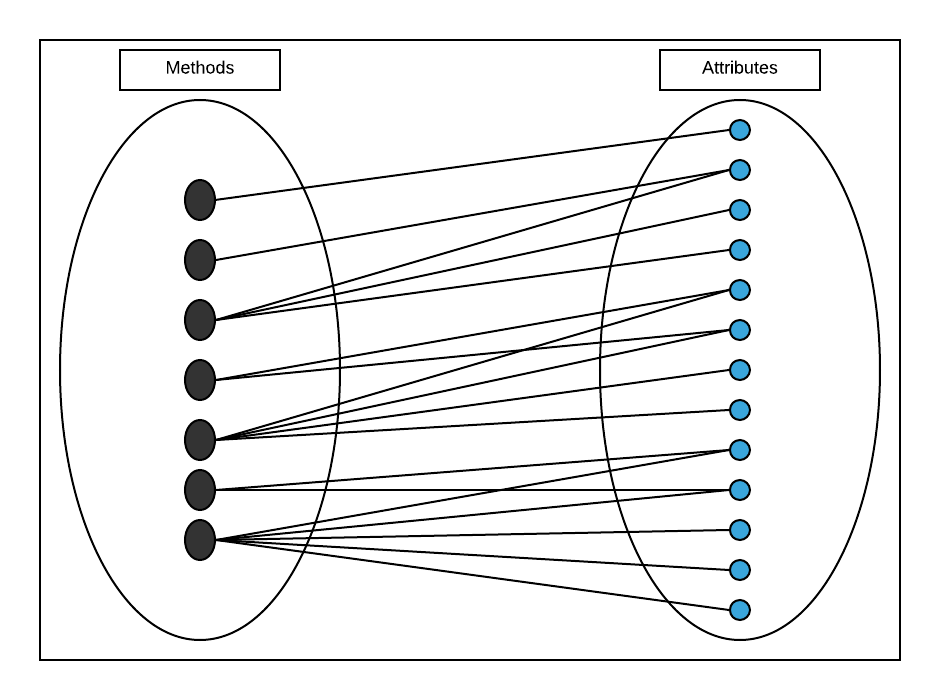
\includegraphics[width=\columnwidth]{Blank_Diagram__1_.png}
		\caption{Scatter Plot of WMC and Rank}
		\label{fig:figure}
		\end{center}
	\end{figure}
Total attribute access = 18\\
Number of methods = 7\\
Number of attributes = 13\\
\textbf{$LCOM^*$ = 0.93} \\
Most of the methods had access to attributes which is an indicator of low coupling. Low $LCOM^*$ is a positive to quality attributes like analyzability, modifiability and testability. \\
\subsection{Coupling Factor (CF)}
CF is used for measuring the coupling between classes excluding the coupling due to Inheritance. It can be used to measure the size of the relationship between two classes. It can be computed as the ratio of of the possible number of couplings in the software to the actual number of couplings not imputable to Inheritance. \\
\begin{equation*}
CF = \frac{\sum_{i=1}^{n}(\sum_{j=1}^n IsClient(C_i,C_j))}{n^2 - n}
\end{equation*}
where,\\ 
Numerator is the actual number of couplings and denominator is the maximum possible      couplings.\\
CF = $\frac{3}{42}$ \\
\textbf{CF = 0.07}\\
Low Coupling Factor is a \textbf{positive to maintainability and testability} but it is a \textbf{negative to reusability}.\\
\section{Physical SLOC and Logical SLOC}
The major classifications of source lines of code are Physical SLOC and Logical SLOC. The definition will be different for both the measurements.\cite{5} \\
\subsection{Physical SLOC}
It is actually the measure of the number of lines in the text format available in a particular program of the source code and it will take commented lines and blank lines into consideration.\\
\subsection{Logical SLOC}
In this case, it will measure only the statements or conditions which are going to be executed from the source code of a program. The statements or conditions depend on the programming language, for example: In C program, every statement will be delimited with (;).
Hence count is based on terminators available in the code. If we compare both Physical and Logical SLOC, Physical SLOC is very easier to describe and measure the style convention according to the language. The measurement of logical SLOC is irrelevant to formatting and styling conventions.
\begin{figure}[H]
		% Center the figure.
		\begin{center}
		% Include the eps file, scale it such that it's width equals the column width. You can also put width=8cm for example...
		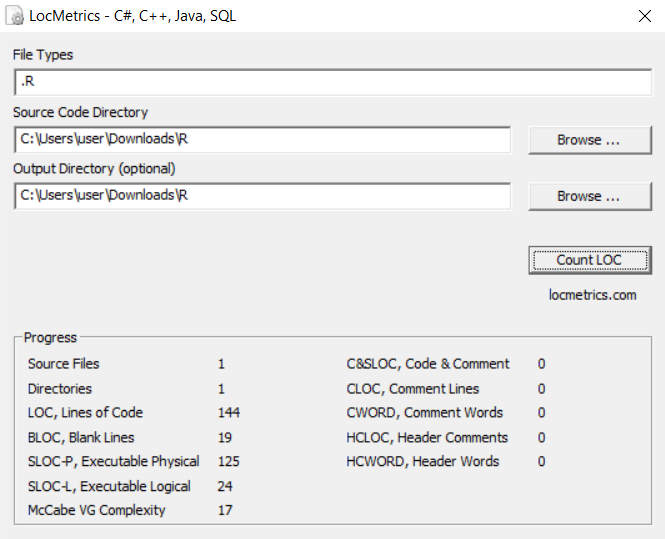
\includegraphics[width=\columnwidth]{LOC.PNG}
		% Create a subtitle for the figure.
		\caption{SLOC using LocMetrics}
		% Define the label of the figure. It's good to use 'fig:title', so you know that the label belongs to a figure.
		\label{fig:figure}
		\end{center}
	\end{figure}
The \textbf{Logical SLOC = 24} using a tool called \textbf{LocMetrics}.\\


\begin{figure}[H]
		\begin{center}
		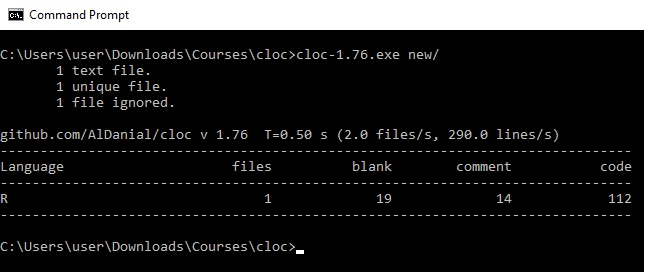
\includegraphics[width=\columnwidth]{CLOC.jpg}
		\caption{SLOC using CLOC}
		\label{fig:figure}
		\end{center}
	\end{figure}
After analyzing our source code using two tools namely, LocMetrics and CLOC whose results are in Figure 9 and Figure 10 respectively, it is shown that both the tools have some drawbacks. Eventhough CLOC computes the SLOC value appropriately, it cannot compute Physical SLOC and Logical SLOC separately.LocMetrics is good comparatively as it can distinguish between physical and logical SLOC but it cannot identify the comments in our source code.\\
We have analyzed our source code manually and the results are as follows \\
\begin{table}[H]
\centering
\begin{tabular}{| >{\centering\arraybackslash}m{2in} | >{\centering\arraybackslash}m{1in} |  >{\centering\arraybackslash}m{1in} |  >{\centering\arraybackslash}m{1in} |  >{\centering\arraybackslash}m{1in} |}
\hline 
\textbf{Function} & \textbf{LOC} & \textbf{SLOC-P} & \textbf{SLOC-L} & \textbf{MVG} \\[8pt]
  \hline
 findMin <- function(x) & 8 & 8 & 2 & 2 \\[8pt]
  \hline
 findMax <- function(x) & 8 & 8 & 2 & 2 \\[8pt] 
 \hline
  calmode <- function(x & 26 & 26 & 6 & 7 \\[12pt]
  \hline
 sortdata <- function(x) & 12 & 12 & 7 & 3 \\[8pt]
  \hline
  findmedian <- function(x) & 17 & 17 & 3 & 1  \\[8pt]
  \hline
  calmean <- function(x) & 9 & 9 & 2 & 1 \\[8pt]
  \hline
  calsd <- function(x) & 10 & 10 & 2 & 1 \\[8pt]
  \hline
\end{tabular} 
\label{my-label}
\caption{LOC Values for each function}
\end{table}
\section{Correlation Coefficient}
Scatter Plot provides greater understanding between two variables. In order to understand the association between variable, We plotted historical data in Scatter Plot using Microsoft Excel. It helped us to understand and analyze precisely.\cite{8} \\ \\
\begin{table}[H]
\centering
\begin{tabular}{| >{\centering\arraybackslash}m{1in} | >{\centering\arraybackslash}m{1in} | >{\centering\arraybackslash}m{1in} | >{\centering\arraybackslash}m{1in} |>{\centering\arraybackslash}m{1in} ||>{\centering\arraybackslash}m{1in} |}
\hline 
  \textbf{WMC($x_i$)} & \textbf{Rank($x_i$)} & \textbf{SLOC($y_i$)} & \textbf{Rank($y_i$)} &\textbf{$d_i$} &\textbf{$d_i^2$} \\[8pt]
  \hline
  1 & 1 & 31 & 1 & 0 & 0 \\[8pt]
  \hline
  50 & 7 & 184 & 8 & -1 & -1 \\[8pt]
  \hline
  32 & 5 &90 & 4 & 1 & 1 \\[8pt]
  \hline
  51 & 8 & 137 & 6 & 1 & 1 \\[8pt]
  \hline
  245 & 10 & 1128 & 10 & 0 & 0 \\[8pt]
  \hline
  34 & 6 & 142 & 7 & -1 & 1 \\[8pt]
  \hline
  73 & 9 & 549 & 9 & 0 & 0 \\[8pt]
  \hline
  19 & 2 & 63 & 2 & 0 & 0 \\[8pt]
  \hline
  31 & 4 & 108 & 5 & -1 & 1 \\[8pt]
  \hline
  21 & 3 & 86 & 3 & 0 & 0 \\[8pt]
  \hline
  23 &  & 24 &  &  &  \\[8pt]
  \hline
\end{tabular}
\label{my-label}
\caption{Historic Data}
\end{table}
First, we are analyzing the association of WMC and SLOC of our historic data from Table 6. \\
\begin{figure}[!hbt]
		% Center the figure.
		\begin{center}
		% Include the eps file, scale it such that it's width equals the column width. You can also put width=8cm for example...
		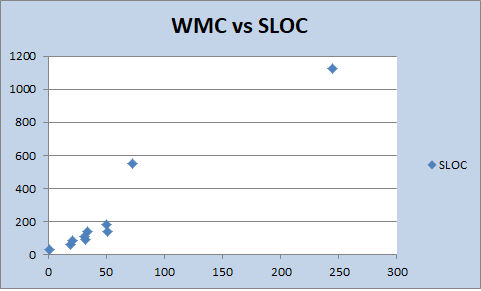
\includegraphics[width=\columnwidth]{Scatter1.png}
		% Create a subtitle for the figure.
		\caption{Scatter Plot of WMC and SLOC}
		% Define the label of the figure. It's good to use 'fig:title', so you know that the label belongs to a figure.
		\label{fig:figure}
		\end{center}
	\end{figure}
From Figure 12, it is evident that SLOC and WMC have a positive association. With the increase in value of SLOC, there will be a corresponding increase in the value of WMC.
\subsection{Correlation Coefficient}
From the historical data, we have ranks for WMC and SLOC. Now, we can determine ranks of our project using our SLOC and WMC value, which in turn helps us to find the correlation coefficient. \\
\subsubsection{WMC vs Rank}
We plotted the Scatter plot for WMC and Rank to find the rank value for our project.
\begin{figure}[!hbt]
		% Center the figure.
		\begin{center}
		% Include the eps file, scale it such that it's width equals the column width. You can also put width=8cm for example...
		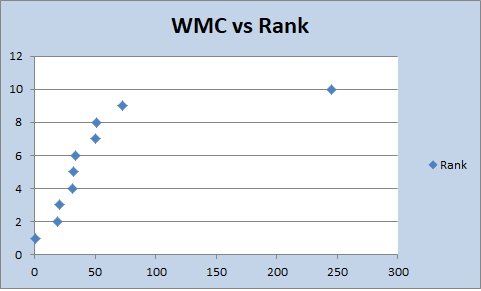
\includegraphics[width=\columnwidth]{Scatter2.png}
		% Create a subtitle for the figure.
		\caption{Scatter Plot of WMC and Rank}
		% Define the label of the figure. It's good to use 'fig:title', so you know that the label belongs to a figure.
		\label{fig:figure}
		\end{center}
	\end{figure}
In Figure 13, we are comparing WMC and Rank. So, we projected a line across the x-axis where x = 23 on this graph. We got an intersection at y-axis where y = 3.5. Rank for our project is 3.5.
\subsubsection{SLOC vs Rank}
\begin{figure}[!hbt]
		% Center the figure.
		\begin{center}
		% Include the eps file, scale it such that it's width equals the column width. You can also put width=8cm for example...
		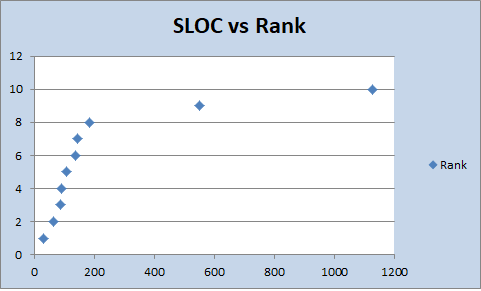
\includegraphics[width=\columnwidth]{Scatter3.png}
		% Create a subtitle for the figure.
		\caption{Scatter Plot of SLOC and Rank}
		% Define the label of the figure. It's good to use 'fig:title', so you know that the label belongs to a figure.
		\label{fig:figure}
		\end{center}
	\end{figure}
    
In Figure 13, we are comparing SLOC and Rank. We projected a line across the x-axis where x = 24 on this graph. We got an intersection at y-axis where y = 0.7. Rank is 0.7. 
\subsubsection{Finding Correlation Coefficient}
To find the correlation coefficient value, we are using Spearman's Rank Correlation Coefficient as our values are not normally distributed. The data is ranked in ascending order.\cite{7} 
\begin{equation*}
r_s = 1-{\frac{6\sum_{i=1}^n{d_i^2}}{n^3-n}}
\end{equation*}
\begin{table}[!hbt]
\centering
\begin{tabular}{| >{\centering\arraybackslash}m{1in} | >{\centering\arraybackslash}m{1in} | >{\centering\arraybackslash}m{1in} | >{\centering\arraybackslash}m{1in} |>{\centering\arraybackslash}m{1in} |>{\centering\arraybackslash}m{1in} |}
\hline 
  \textbf{WMC($x_i$)} & \textbf{Rank($x_i$)} & \textbf{SLOC($y_i$)} & \textbf{Rank($y_i$)} &\textbf{$d_i$} &\textbf{$d_i^2$} \\[8pt]
  \hline
  1 & 1 & 31 & 1 & 0 & 0 \\[8pt]
  \hline
  50 & 7 & 184 & 8 & -1 & 1 \\[8pt]
  \hline
  32 & 5 &90 & 4 & 1 & 1 \\[8pt]
  \hline
  51 & 8 & 137 & 6 & 2 & 4 \\[8pt]
  \hline
  245 & 10 & 1128 & 10 & 0 & 0 \\[8pt]
  \hline
  34 & 6 & 142 & 7 & -1 & 1 \\[8pt]
  \hline
  73 & 9 & 549 & 9 & 0 & 0 \\[8pt]
  \hline
  19 & 2 & 63 & 2 & 0 & 0 \\[8pt]
  \hline
  31 & 4 & 108 & 5 & -1 & 1 \\[8pt]
  \hline
  21 & 3 & 86 & 3 & 0 & 0 \\[8pt]
  \hline
  23 & 4.5 & 24 & 0.7 & 3.8 & 14.44 \\[8pt]
  \hline
\end{tabular} 
\caption{Our Project Data}
\end{table}
After substituting our values from Table 7 in equation, we obtain our correlation coefficient value. \\
\begin{equation*}
r_s = 1-\frac{134.64}{990}\\
r_s = 0.997 \\
\end{equation*}
Our correlation coefficient value is close to 1. Hence, it indicates a strong positive correlation. This data can be stored and used for future projects.\\ \\
\section{Conclusion} 
By analyzing the data which is generated randomly, we were able to deduce and compare measurements processed on the metrics which can be used to improve the customer satisfaction. We also realized the significance of having historical data to derive future estimation as well as deciding the threshold value, which can be helpful to satisfy our business goal. \\
\section{Acknowledgement}
The inclusion of an image in this document and the usage of mathematical equations related to metrics are for academic purpose, and its use is hereby acknowledged.  

\section{Contribution Distribution}
\subsection{Project Work distribution}
\begin{enumerate}
  
  \item Goal finalization, decision making and brainstorming.
   \begin{itemize}
     \item Total Contribution of each member.
   \end{itemize}
      
   \item UseCase Modeling of part A
   \begin{itemize}
     \item Rahul Reddy Ayyapaneni, Divyeshkumar Balar
   \end{itemize}
   
   \item Cost Estimation using COCOMO \& UCP
   \begin{itemize}
     \item Rahul Reddy Ayyapaneni, Priyanka Anantha Padmanabhan
   \end{itemize}
   
   \item R Programming, testing, documentation
   \begin{itemize}
     \item Maryam Ansari Sadrabadi, Rahul Reddy Ayyapaneni, Priyanka Anantha Padmanabhan
   \end{itemize}
   
      \item Cyclometic Complexity measurement, Flow Chart making
   \begin{itemize}
     \item Divyeshkumar Balar, Rahul Reddy Ayyapaneni
   \end{itemize}
   
      \item Calculation of WMC, CF and LCOM* for source code
   \begin{itemize}
     \item Nikitha Papani, Divyeshkumar Balar, Mitra Azari Sissi, Rahul Reddy Ayyapaneni
   \end{itemize}
   
      \item Physical and Logical SLOC Calculation
   \begin{itemize}
     \item Rahul Reddy Ayyapaneni
   \end{itemize}
   
   \item Scatter Plot analysis on correlation
   \begin{itemize}
     \item Priyanka Anantha Padmanabhan, Nazanin AhmadyShahpourAbady
   \end{itemize}
\end{enumerate}

\subsection{Documentation}
\begin{enumerate}
   \item LaTex Documentation
   \begin{itemize}
     \item Divyeshkumar Balar, Rahul Reddy Ayyapaneni, Nikitha Papani, Priyanka Anantha Padmanabhan
   \end{itemize}
   \item validation \& verification
   \begin{itemize}
     \item Divyeshkumar Balar, Rahul Reddy Ayyapaneni, Nikitha Papani, Priyanka Anantha Padmanabhan
   \end{itemize}
\end{enumerate}
	

\section{Glossary}
\textbf{A} \\ 
\textbf{A}cknowledge – acceptance or admitting something \\
\textbf{A}ccuracy - the degree to which the result of a measurement, calculation, or specification conforms to the correct value or a standard \\
\textbf{A}ctor - The actor can be a human or other external system \\
\textbf{A}ppend- add (something) as an attachment or supplement. \\
\textbf{A}nalyze- discover or reveal (something) through detailed examination \\
\textbf{A}ssigned- designate or set (something) aside for a specific purpose. \\
\textbf{A}verage- a number expressing the central or typical value in a set of data, in particular the mode, median, or (most commonly) the mean, which is calculated by dividing the sum of the values in the set by their number\\ \\
\textbf{B} \\
\textbf{B}eneficial - favorable \\ \\
\textbf{C}\\
\textbf{C}omplex- consisting of many different and connected parts.\\
\textbf{C}oncurrent- existing, happening, or done at the same time\\
\textbf{C}omputed- calculate\\
\textbf{C}OCOMO - Constructive Cost Model.\\
\textbf{C}ohesion – forming an united whole\\
\textbf{C}ommercial- making or intended to make a profit.\\
\textbf{C}orrelation- a mutual relationship or connection between two or more things.\\
\textbf{C}oupling- the pairing of two items.\\
\textbf{C}oefficient- a numerical or constant quantity placed before and multiplying the variable in an algebraic\\ \\
\textbf{D}\\
\textbf{D}ataframe - a collection of related sets of information that is composed of separate elements but can be manipulated as a unit by a computer.\\
\textbf{D}efect- imperfection\\
\textbf{D}ependability – measure of system’s availability, reliability\\
\textbf{D}escriptive - describe\\
\textbf{D}isplay- performance\\
\textbf{D}istributed systems- many independent computers linked by a network.\\
\textbf{D}RE – Defect Removal Efficiency\\
\textbf{D}S - Descriptive Statistics \\ \\
\textbf{E}\\
\textbf{E}CF – Environment Complexity Factor\\
\textbf{E}stimated- roughly calculate or judge the value\\
\textbf{E}ffort- a vigorous or determined attempt\\
\textbf{E}valuate- form an idea of the amount, number, or value of; assess.\\
\textbf{E}mbedded-Implant.\\
\textbf{E}xecuted- perform\\
\textbf{E}dges - Line connecting two nodes.\\ \\
\textbf{G}\\
\textbf{G}QM - Goal, Question, Metrics.\\ \\
\textbf{I}\\
\textbf{I}nspection - careful examination\\
\textbf{I}nstability -  low stability\\ \\
\textbf{L}\\
\textbf{L}OD – Lack of Documentation\\
\textbf{L}COM – Lack of Cohesion\\ \\
\textbf{M}\\
\textbf{M}ean - In mathematics and statistics, the arithmetic mean, or simply the mean or average when the context is clear, is the sum of a collection of numbers divided by the number of numbers in the collection.\\
\textbf{M}edian - The middle number.\\
\textbf{M}ode - The number which appears most often in a set of numbers.\\ \\
\textbf{O}\\
\textbf{O}OD - Object oriented design.\\
\textbf{O}rganic - denoting a relation between elements of something such that they fit together harmoniously as necessary parts of a whole.\\ \\
\textbf{P}\\
\textbf{P}roductivity - Productivity is an average measure of the efficiency of production.\\
\textbf{P}erformance - the action or process of carrying out or accomplishing an action, task, or function\\
Portable - able to be easily carried or moved, especially because of being a lighter and smaller version than usual\\ \\
\textbf{R}\\
\textbf{R}eusability - In computer science and software engineering, reusability is the use of existing assets in some form within the software product development process.\\ \\
\textbf{S}\\
\textbf{S}emi-detached - partially separate.\\
\textbf{S}tandard Deviation- In statistics, the standard deviation (SD, also represented by the Greek letter sigma σ or s) is a measure that is used to quantify the amount of variation or dispersion of a set of data values\\
\textbf{S}ystem - the programs and other operating information used by a computer that considered.\\
\textbf{S}ignificant - sufficiently great or important to be worthy of attention.\\
\textbf{S}cenarios - a postulated sequence or development of events. \\ \\
\textbf{T}\\
\textbf{T}CF – Technical Complexity Factor\\ \\
\textbf{U}\\
\textbf{U}ML  -Use case modeling.\\
\textbf{U}CP - Use case point.\\
\textbf{U}UCP - Unadjusted use case points.\\
\textbf{U}AW - Unadjusted use case actor weight.\\ \\
\textbf{V}\\
\textbf{V}ariability- not consistent or having a fixed pattern.\\
\textbf{V}ariance- In probability theory and statistics, variance measures how far a set of numbers are spread out. A variance of zero indicates that all the values are identical.\\
\textbf{V}ariables- an element, feature, or factor that is liable to vary or change\\ \\

\begin{thebibliography}{12}

\bibitem{1}  {P. Kamthan, "INTRODUCTION TO SOFTWARE MEASUREMENT". https://users.encs.concordia.ca/kamthan/courses/soen6611/software measurement introduction.pdf}.

\bibitem{2}  {P. Kamthan, "INTRODUCTION TO FRAMEWORKS FOR
SOFTWARE MEASUREMENT". https://users.encs.concordia.ca/kamthan/courses/soen6611/software measurement frameworks introduction.pdf}

\bibitem{3}  {P. Kamthan, "INTRODUCTION TO
SOFTWARE PROJECT COST ESTIMATION". https://users.encs.concordia.ca/kamthan/courses/soen6611/software project cost estimation introduction.pdf}

\bibitem{4}  {P. Kamthan, "THE ESTIMATION OF EFFORT BASED ON USE CASES". https://users.encs.concordia.ca/kamthan/courses/soen6611/effort estimation use cases.pdf}

\bibitem{5}  {P. Kamthan, "LENGTH OF SOURCE CODE". https://users.encs.concordia.ca/kamthan/courses/soen6611/source code length.pdf}

\bibitem{6}  {P. Kamthan, "CONTROL FLOW STRUCTURE OF SOURCE CODE". https://users.encs.concordia.ca/kamthan/courses/soen6611/source code control flow structure.pdf}

\bibitem{7}  {P. Kamthan, "INTRODUCTION TO ANALYSIS OF
SOFTWARE MEASUREMENT DATA". https://users.encs.concordia.ca/kamthan/courses/soen6611/software measurement data analysis.pdf}

\bibitem{8}  {P. Kamthan, "METRICS FOR PACKAGES IN OBJECT-ORIENTED DESIGN ". https://users.encs.concordia.ca/kamthan/courses/soen6611/ood metrics packages.pdf}

\bibitem{9}  {P. Kamthan, "METRICS FOR CLASSES IN OBJECT-ORIENTED DESIGN".https://users.encs.concordia.ca/kamthan/courses/soen6611/ood metrics classes.pdf}

\bibitem{10}  {"Software Quality Metrics". http://www.arisa.se/compendium/node88.html/}. 

\bibitem{11} {CSAT VS. NPS VS. CES: YOUR GUIDE TO CUSTOMER SUPPORT SCORES} {https://www.taskus.com/blog/csat-vs-nps-vs-ces-guide-customer-support-scores/}.

\bibitem{12} {F. Eric, H. Morton, H. Kasper "Measuring Usability: Are Effectiveness, Efficiency, and Satisfaction Really Correlated?"} {https://dl.acm.org/citation.cfm?id=332455}

\bibitem{13} {"16 metrics to ensure MobileAppSuccess". https://www.appdynamics.com/media/uploaded-files/1432066155/white-paper-16-metrics-every-mobile-team-should-monitor.pdf}.

\bibitem{14} {P. Ramachandran, S. Adve et. all"Metrics for Lifetime Reliability"}

\end{thebibliography} 

\end{document}
